The results exposed here are for the PTW TM33054 magnesium chamber with a layer of \textbf{hydromagnesite} on all the magnesium surfaces. In this section, it is intended to study the differences in the response when a layer of corrosion of the mentioned composite is present. For this purpose, the MCNP simulation tally the dose absorbed by the argon gas.  The simulations have been conducted using the geometry setup of Figure \ref{fig:Simulated PTW (left) and closeup (right)}:

\begin{figure}[!h]
\centering
\begin{minipage}{0.5\textwidth}
    %\renewcommand{\thefigure}{A} % Set the label of the first figure to A
    \centering
    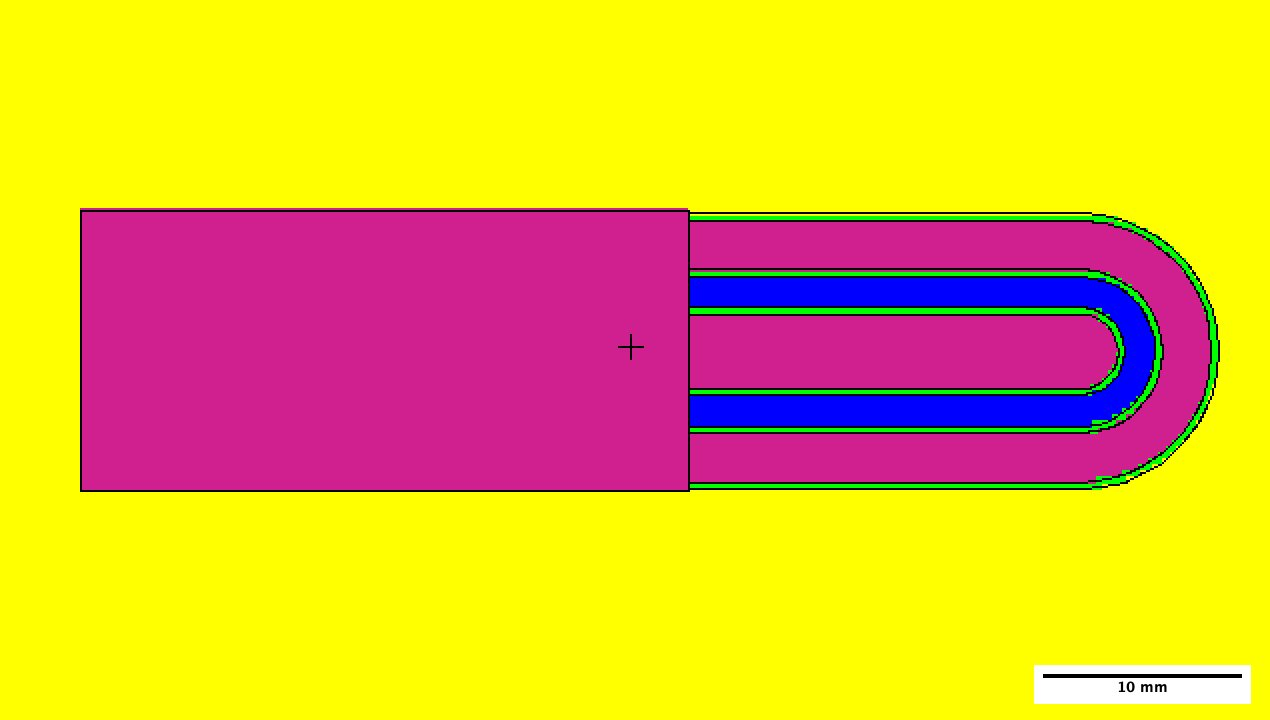
\includegraphics[width=\linewidth]{Master Thesis Manuel Galdon/figures/IC_scale.jpg}
    %\caption{Simulated PTW chamber}
    \label{fig:IC}
\end{minipage}
\hfill
\begin{minipage}{0.4\textwidth}
    \centering
    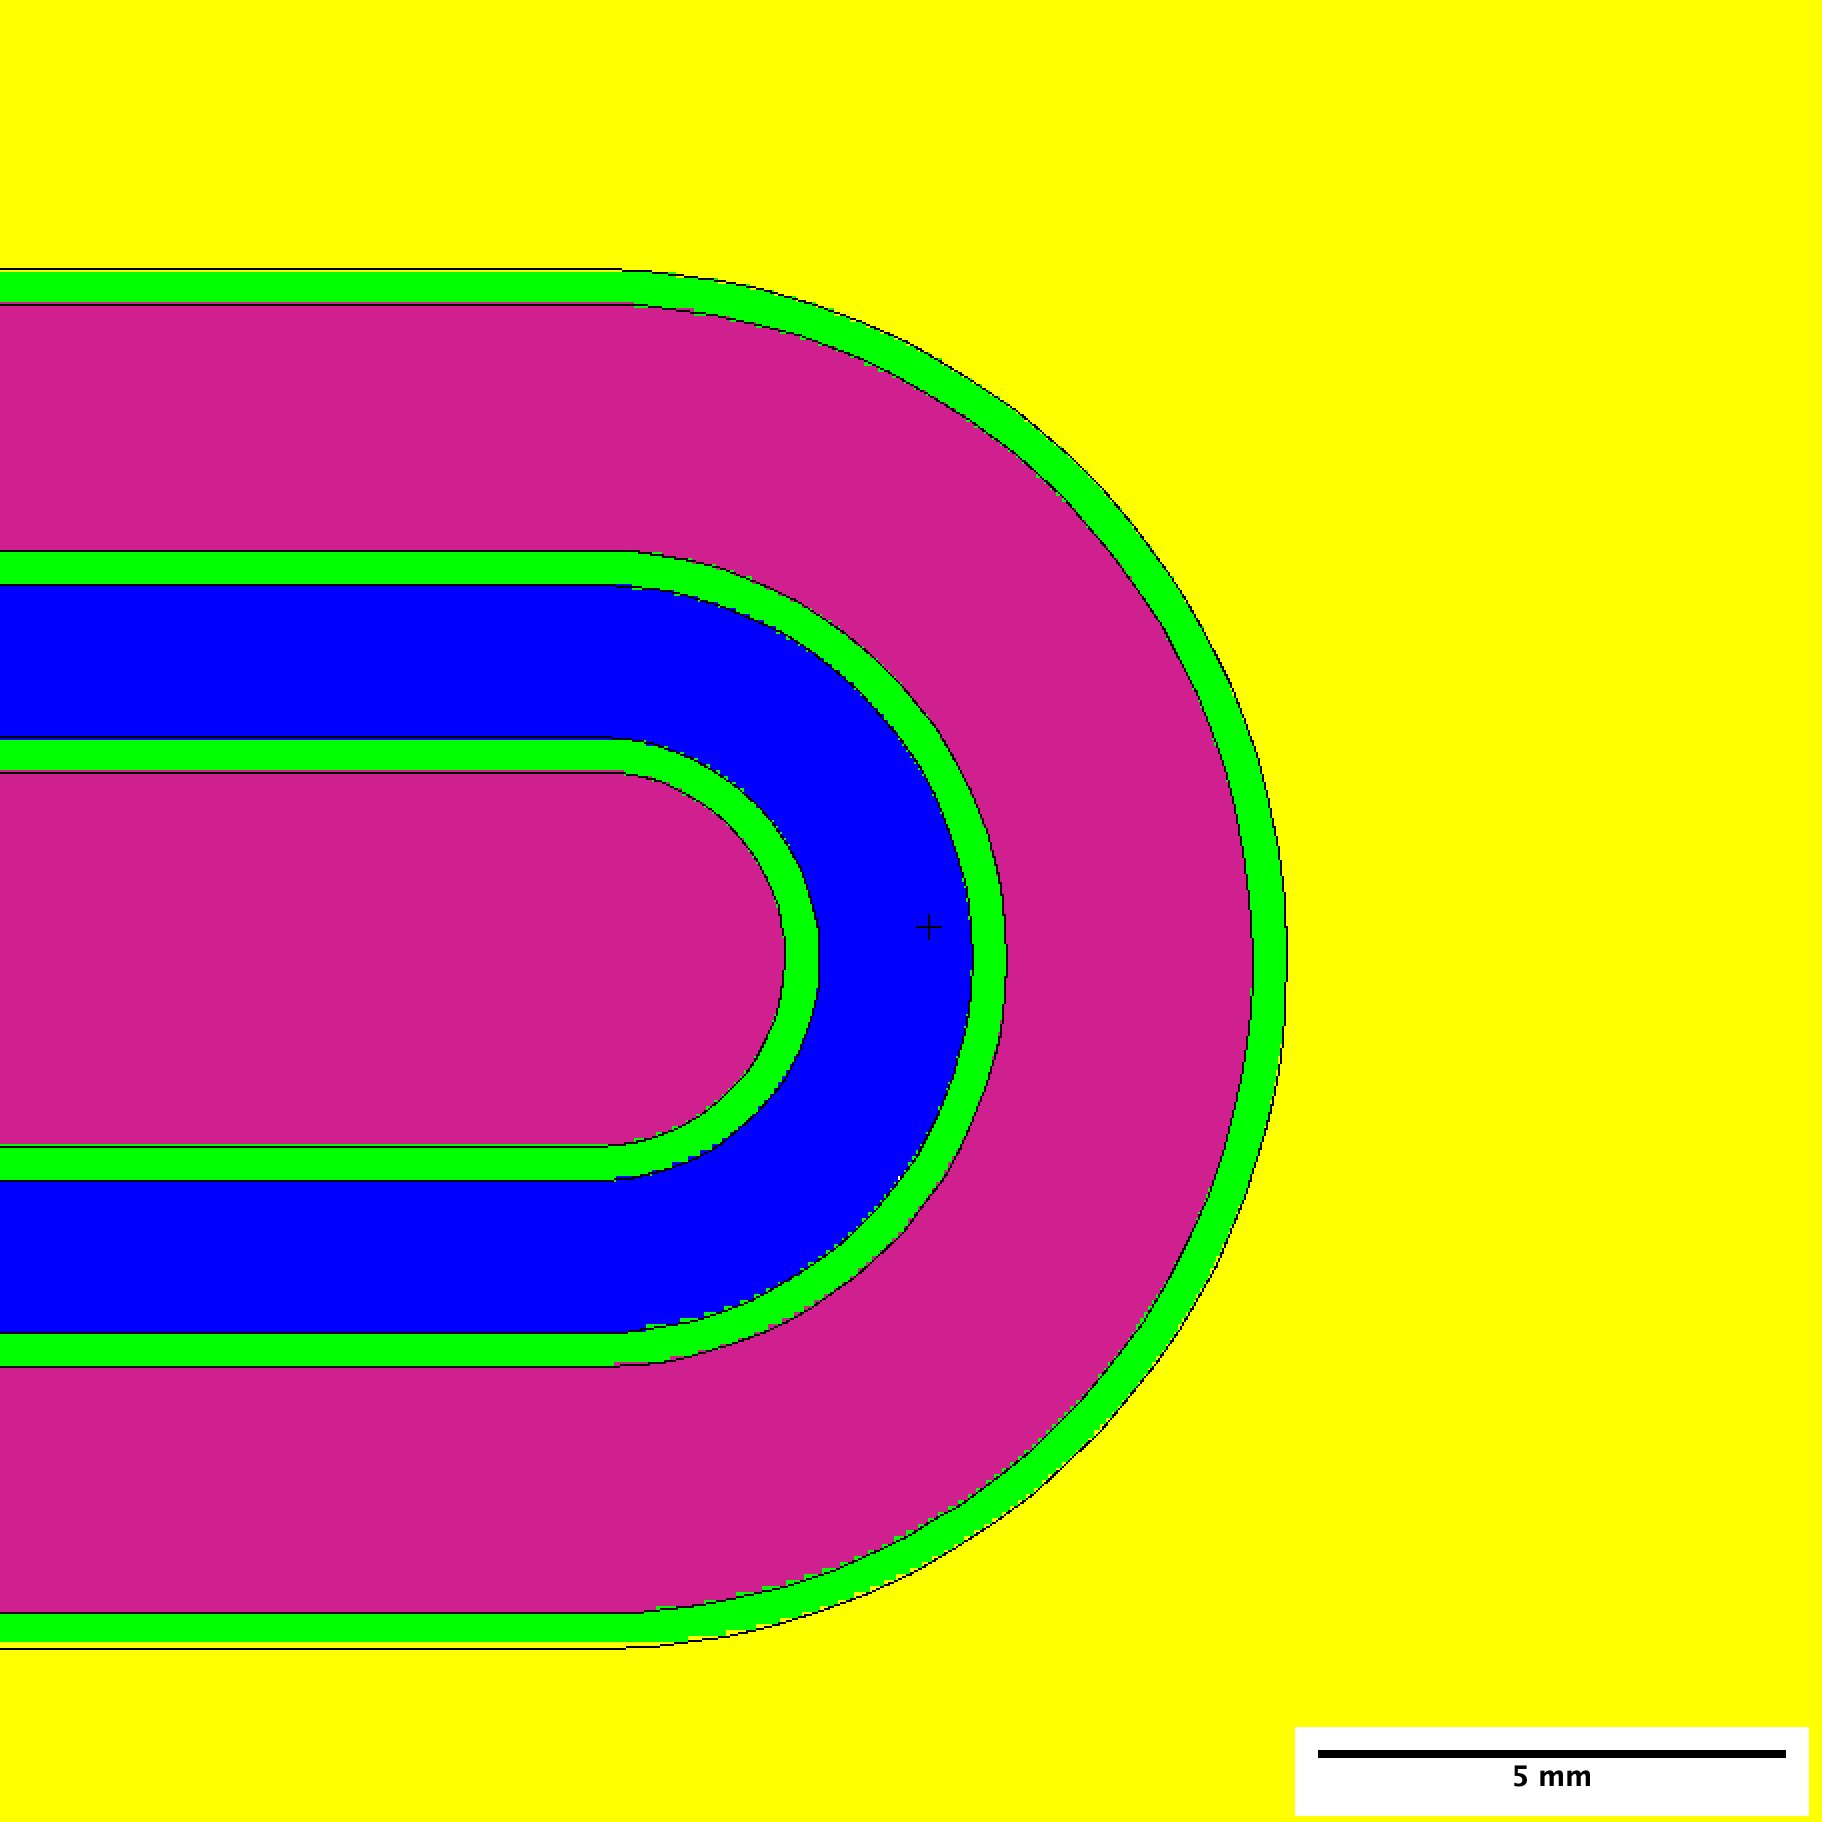
\includegraphics[width=\linewidth]{Master Thesis Manuel Galdon/figures/IC closeup_scale.jpg}
    %\caption{Close-up of PTW chamber}
    %\label{fig:IC closeup}
\end{minipage}
\caption{Simulated PTW chamber (left) and a close-up of the tip of the chamber (right). In the close-up, it is noticeable that a layer of hydromagnesite, shown in green, is added to the surface of the anode and to the inner part of the wall. The scale bar has been placed at the bottom of both images. }
\label{fig:Simulated PTW (left) and closeup (right)}
\end{figure}

\newpage

In the simulation that includes the corrosion layer, the source of radiation is the MEDAPP source. The simulation is also run using the same source, but removing the photon contribution. The purpose of it is to compare the response of the device without the influence of gamma radiation.

The density of argon is, according to the \textit{National Institute of Standards and Technology} \cite{ESTAR}, equal to 1.66 \unit{\mg\per\cubic\cm}. For hydromagnesite, the average density is 2.18 \unit{\g\per\cubic\cm} according to the \textit{Mineralogy Database} \cite{MineralogyDatabase}.
Furthermore, the simulation also runs with a material that is a mixture of hydromagnesite and a small amount of water. This is done to consider the case in which a certain amount of atmospheric water is dissolved into the hydromagnesite. The high interaction probability of neutrons with hydrogen can significantly affect the reading of the chamber. Therefore, it is of interest to consider this case as well.
In MCNP, the mixed material of hydromagnesite and water has been simulated by calculating respectively the molecular fraction of each element according to the desired concentration of water. The molecular weight that is used to calculate the molecular fraction when the mineral is mixed with water is also taken from the database \cite{MineralogyDatabase}.

\subsection{MEDAPP Source with a Hydromagnesite Corrosion Layer}

The source of radiation used in this simulation is the \textbf{MEDAPP} source accounting for the contribution of \textbf{neutrons and photons} and the total number of particles simulated is $10^8$. The reason for this decision is the trade-off between the computational time and the statistical error of the results: while a higher number of particles will sharpen-up the results, it will slow down the execution dramatically beyond $10^8$ particles. Finally, the \textbf{thickness} has been set to \textbf{0.37} \textbf{mm}.
The density of hydromagnesite decreases slightly as the fraction of water increases. This has been taken into account in the simulation and the density has been set according to the next table for each case: 

\begin{table}[!h]
\centering
\begin{tabular}{|c|c|}
\hline
\rowcolor[HTML]{A9D9C6} 
\% of water & Density {[}\unit{\gram\per\cubic\centi\meter}{]} \\ \hline
0           & 2.18                                  \\ \hline
1           & 2.17                               \\ \hline
2           & 2.16                               \\ \hline
3           & 2.14                               \\ \hline
\end{tabular}
\caption{Density of the hydromagnesite composite accounting for a percentage of water.}
\end{table}

Figure \ref{fig:PTW-33053 with hydromagnesite. Tally +F6} shows the tally +F6, which accounts for the total dose deposited by all particles, against the density of the argon gas. The same tally \textbf{without} any corrosion layer is included in the same figure to compare. 

\begin{figure}[!h]
  \centering
  \includegraphics[width=0.8\textwidth]{Master Thesis Manuel Galdon/figures/corrosion/Hydromagnesite/Neutrons and Photons/+F6.jpg}
  \caption{Simulation of PTW TM33054 with a 0.37 \unit{\milli\meter} thick layer of hydromagnesite on all magnesium surfaces. Tally +F6. In the legend the fraction of water is stated in percentages.}
  \label{fig:PTW-33053 with hydromagnesite. Tally +F6}
\end{figure}
\newpage
From the graph, it is evident that as the density of argon increases, there is a general downward trend in the deposited dose. Here, the downward trend is caused due to the increase of total mass in the sensitive region since the relationship between dose and mass is $D = \frac{E}{m}$, where $D$ is the dose, $E$ the energy and $m$ the mass of the gas. The presence of a higher concentration of water in the layer leads to a greater generation of secondary protons and hence to a deposition of dose.

The energy deposited in the sensitive region where the argon gas is located is a measure of interest. To come up with that plot, the energy deposition is calculated as $Dose$ x $mass$, where the dose is in \unit{\mega\electronvolt} and the mass is the mass of the argon in \unit{\gram}, which has been calculated by $\rho$ x V. The density $\rho$ is the density of the gas in \unit{\gram\per\cubic\centimeter}, and the volume V has been read from MCNP as 0.79 \unit{\cubic\cm}. The total energy deposition is, then:
\newpage
\begin{figure}[!h]
  \centering
  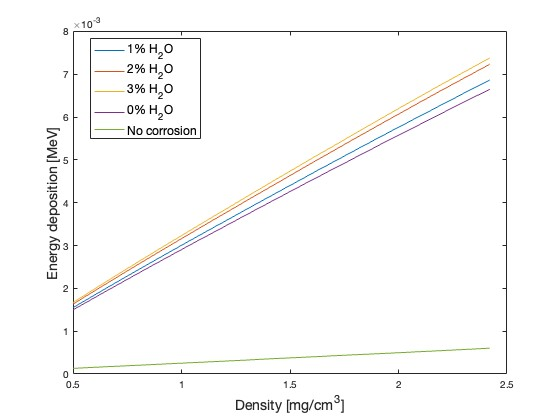
\includegraphics[width=0.8\textwidth]{Master Thesis Manuel Galdon/figures/corrosion/Hydromagnesite/Neutrons and Photons/Energy deposition.jpg}
  \caption{Energy deposition in the sensitive region of the PTW TM33054 chamber with a  hydromagnesite layer.}
  \label{fig:PTW-33053 with hydromagnesite. Energy deposition}
\end{figure}

The relationship between the argon mass and the density is linear. Therefore, the \textbf{total} energy deposition shows an increasing trend.

To compare the energy absorption further, the data presented in the Figure \ref{fig:PTW-33053 with hydromagnesite. Energy deposition} are fitted linearly and the slope of each function is calculated. In the next table, the slopes are presented for each simulation: 

\begin{table}[!h]
\centering
\begin{tabular}{|c|c|}
\hline
\rowcolor[HTML]{A9D9C6} 
\% of water & Slope [10^{-3}]\\ \hline
No corrosion           & 2.6\\ \hline
0           & 3.6                                \\ \hline
1           & 3.7                               \\ \hline
2           & 3.7                               \\ \hline
3           & 3.8                               \\ \hline
\end{tabular}
\caption{Slope comparison of the linear fit for the energy deposition of the MEDAPP source in PTW TM33054. No corrosion corresponds to the simulation of the chamber where no corrosion layer has been included.}
\label{table: Slope comparison for MEDAPP source at the energy deposition}
\end{table}
The slope increases between 1 and 4 $\%$ per fraction of water. The minimum increase of slope with regards to the simulation without a corrosion layer is more than 20 $\%$. In this result it is shown that the presence of a corrosion layer does influence the absorbed dose, although it is not necessary for the gas to absorb any amount of the energy.


Following the energy deposition, the contribution of the \textbf{neutrons} to the total dose is:
\begin{figure}[!h]
  \centering
  \includegraphics[width=0.8\textwidth]{Master Thesis Manuel Galdon/figures/corrosion/Hydromagnesite/Neutrons and Photons/neutrons.jpg}
  \caption{Dose delivered by neutrons in the sensitive region of the PTW TM33054 chamber with a 0.37 \unit{\milli\meter} thick hydromagnesite layer.}
  \label{fig:PTW-33053 with hydromagnesite. Neutron dose deposition}
\end{figure}

The neutron contribution is perhaps one of the lowest of this simulation. The value barely changes with the fraction of water. However, the dose deposited is about $1\%$ lower in the case of the simulation where no corrosion layer has been included. With a dose of the order of $2.2 \cdot 10^{-15}$ \unit{\gray} in presence of corrosion, it is lower than the dose delivered by electrons and photons by a factor of 100, which is presented up next in Figure \ref{fig:IC3305 with hydromagnesite, MEDAPP, electron and proton contribution. Full MEDAPP}. 
\clearpage
Electrons and protons contribute to the dose as follows: 

\begin{figure}[!h]
  \centering
    \centerline{\includegraphics[width=1.22\textwidth]{Master Thesis Manuel Galdon/figures/corrosion/Hydromagnesite/Neutrons and Photons/electrons vs protons.jpg}}
  \caption{Simulation of PTW TM33054 with a 0.37 \unit{\milli\meter} thick layer of hydromagnesite on all magnesium surfaces. Electron and proton contribution.}
  \label{fig:IC3305 with hydromagnesite, MEDAPP, electron and proton contribution. Full MEDAPP}
\end{figure}


Although the lines of the dose for the respective fractions of water appear in the subplots very close to each other (except in the total and proton plot), the sensitive region's behaviour is the same for all kinds of particles except for electrons.
Electrons slightly depend on the fraction of water as they show a variation of roughly 1 $\%$ of the dose delivered. Protons, on the other hand, happen to be more relevant as their dose deposition varies about 5 $\%$ across the fractions of water

However, photons and heavy ions do not play an role in the dose and their contribution is of the order of $10^{-13}$ and $10^{-14}$ \unit{\gray}, respectively. For this reason, their plots are not shown here.

\clearpage
\subsection{Neutron Source with a Hydromagnesite Corrosion Layer}

In this simulation, the contribution of the photons is excluded in MCNP. The source only has the neutron contribution. The number of particles and the thickness of the layer is the same as in the previous simulation. For the neutrons, the energy and probability distribution is exactly the same as in the previous case. The total dose delivered by the source in the sensitive region is plotted in Figure \ref{fig:PTW-33053 with hydromagnesite. Tally +F6. Only neutrons}.

\begin{figure}[!h]
  \centering
  \includegraphics[width=0.8\textwidth]{Master Thesis Manuel Galdon/figures/corrosion/Hydromagnesite/Neutrons/+F6.jpg}
  \caption{Simulation of PTW TM33054 with a 0.37 \unit{\milli\meter} thick layer of hydromagnesite on all magnesium surfaces using the MEDAPP neutron source. Tally +F6. In the legend the fraction of water is stated in percentages.}
  \label{fig:PTW-33053 with hydromagnesite. Tally +F6. Only neutrons}
\end{figure}

The dose is slightly lower in this simulation because of the lack of photons, which also deliver a certain dose and generate secondary particles. The dose delivered in the simulation that has no corrosion layer in notably lower than the rest. The total dose absorbed by the gas in that simulation is about 90 $\%$ lower in absence of photons. This means that neutrons barely interact with the magnesium outer layer, while they do with the hydrogen atoms present in the corrosion layer. Thus, the layer does play a significant role when only neutrons are used as a source.
\newpage

\newpage
The total en energy deposition is also calculated in this simulation and is plotted in Figure \ref{fig:PTW-33053 with hydromagnesite. Energy deposition. Neutrons}.
\begin{figure}[!h]
  \centering
  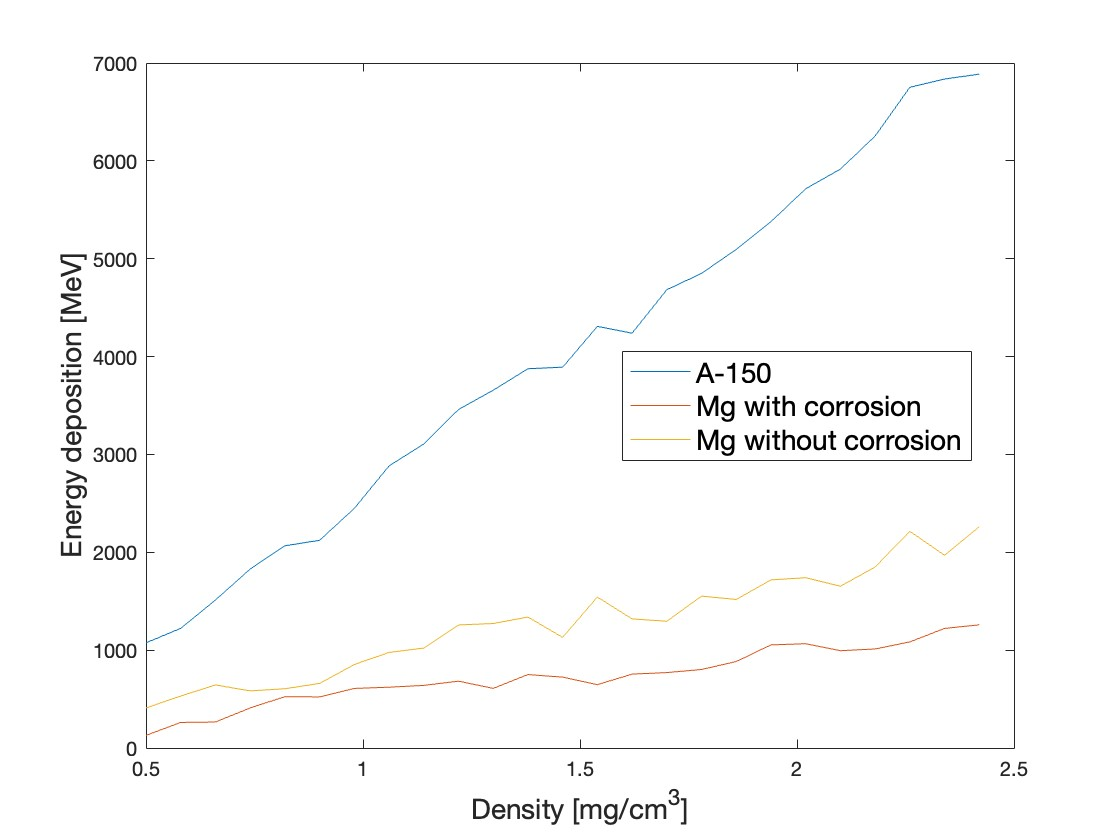
\includegraphics[width=0.8\textwidth]{Master Thesis Manuel Galdon/figures/corrosion/Hydromagnesite/Neutrons/energy deposition.jpg}
  \caption{Energy deposition in the sensitive region of the PTW TM33054 chamber with a  hydromagnesite layer using the MEDAPP neutron source.}
  \label{fig:PTW-33053 with hydromagnesite. Energy deposition. Neutrons}
\end{figure}

As presented the simulation using the complete MEDAPP source, a comparison of the energy absorption for the fractions of water is made using a linear fit. In the next table, the slopes are presented for each simulation: 

\begin{table}[!h]
\centering
\begin{tabular}{|c|c|}
\hline
\rowcolor[HTML]{A9D9C6} 
\% of water & Slope [10^{-3}]\\ \hline
No corrosion           & 0.24\\ \hline
0           & 2.7                                \\ \hline
1           & 2.8                               \\ \hline
2           & 2.9                               \\ \hline
3           & 3.0                               \\ \hline
\end{tabular}
\caption{Slope comparison of the linear fit for the energy deposition of the MEDAPP neutron source in PTW TM33054. No corrosion corresponds to the simulation of the chamber where no corrosion layer is included.}
\label{table: Slope comparison for MEDAPP source at the energy deposition. Neutrons}
\end{table}

Again, the slope increases between 1 and 4 $\%$ per fraction of water. As suggested before, the most significant contrast is observed in the simulation without corrosion, where the slope is about 97 $\%$ lower than in the presence of the layer. The presence of the layer can be regarded as necessary in the case of a neutron source for the chamber to absorb a significant dose.
The contribution of the neutrons, electrons and protons is presented next:

\begin{figure}[!h]
  \centering
    \centerline{\includegraphics[width=0.8\textwidth]{Master Thesis Manuel Galdon/figures/corrosion/Hydromagnesite/Neutrons/neutrons.jpg}}
  \caption{Simulation of PTW TM33054 with a 0.37 \unit{\milli\meter} thick layer of hydromagnesite on all magnesium surfaces using the MEDAPP neutron source. Neutron contribution.}
  \label{fig:IC3305 with hydromagnesite, MEDAPP, neutron contribution. Neutron source}
\end{figure}
As it is expected, the neutron contribution is almost twice as strong as the complete MEDAPP source, in which the chamber is irradiated only with neutrons. 

\clearpage
The electron and proton contribution is shown in the next plot:
\begin{figure}[!h]
  \centering
    \centerline{\includegraphics[width=1.22\textwidth]{Master Thesis Manuel Galdon/figures/corrosion/Hydromagnesite/Neutrons/electrons vs protons.jpg}}
  \caption{Simulation of PTW TM33054 with a 0.37 \unit{\milli\meter} thick layer of hydromagnesite on all magnesium surfaces. Electron and proton contribution.}
  \label{fig:IC3305 with hydromagnesite, MEDAPP, electorn and proton contribution}
\end{figure}

There are almost no protons generated by the neutron source when there is no corrosion layer. The dose of that simulation is of the order of $10^{-17}$ \unit{\gray}.